\chapter[Structuring Machine Learning Projects]{Structuring Machine \\Learning Projects}

%%%
\section{ML Strategy}


%%%%
\subsection{Introduction to ML Strategy}

\subsubsection{Why ML Strategy}

为了提高深度学习系统的准确性,可以尝试以下方法:

\begin{itemize}
    \item 收集更多数据。
    \item 收集更多样化的训练集。
    \item 训练更多轮数。
    \item 尝试不同的优化算法(例如 Adam)。
    \item 添加正则化方法。
    \item 改变网络架构(激活函数、隐藏单元数量等)。
\end{itemize}

本章主要探讨这些方法在什么情况下适合使用。

\subsubsection{Orthogonalization}
\index{Orthogonalization}

\textbf{正交化(Orthogonalization)}是指调整的超参数只对特定的目标有影响,不对其他目标产生影响。
在正交化中,每个控制参数只执行特定任务,不影响其他控制参数,做到“互不干扰”。

对于监督学习系统来说,要表现良好,通常需要调整系统参数以确保下面的四个条件成立:

\begin{enumerate}
    \item 在成本函数上很好地拟合训练集(尽可能接近甚至超过人类水平)。
    \item 在成本函数上很好地拟合开发集。
    \item 在成本函数上很好地拟合测试集。
    \item 在现实世界的真实数据中表现良好。
\end{enumerate}


%%%%
\subsection{Setting Up your Goal}

\subsubsection{Single Number Evaluation Metric}

单一的、明确的、可量化的评估指标可以帮助你快速了解你的模型的性能。
确定一个\textbf{单一数字评估指标(Single Number Evaluation Metric)}是评估深度学习系统性能的重要一步,
有了这个明确的量化标准,可以更方便地比较不同模型的性能,并不断对系统进行迭代改进。

通常,这个指标可以是准确率、mAP、Artificial Analysis Quality Index(人工分析质量指数)等。
在有些情况下,简单的准确率并不足以评估模型的性能。
例如在疾病诊断、欺诈检测等场景中,漏掉一个正例(例如未检测到的疾病或欺诈行为)
可能比误报一个负例(例如错误地将健康人诊断为病人或将合法交易标记为欺诈)的后果要严重得多。
此时,衡量模型正确识别的正例所占比例的\textbf{召回率(Recall)}也十分重要,
这种情况下将准确率和召回率结合起来作为评估指标会更有意义。
结合的方式有多种,例如精确率和召回率的调和平均 \textbf{F1 值(F1 Score)}。

\subsubsection{Satisficing and Optimizing Metric}

指标通常可以分为两类:
\index{Satisficing Metric}
\index{Optimizing Metric}

\begin{enumerate}
    \item \textbf{满足指标(Satisficing Metric)}:指标只需要满足某个阈值,例如单样本运行时间小于 100\,ms;
    \item \textbf{优化指标(Optimizing Metric)}:指标可以量化且越大(小)越好,例如分类准确率。
\end{enumerate}

将所有的优化指标按照某种方式综合起来得到单一数字评估指标,同时让模型满足所有的满足指标,
在这样的基础上不断迭代和优化模型的性能。

\subsubsection{Train/Dev/Test Distributions}
\label{sec:train_dev_test_distributions}

开发集和测试集需要满足相同的分布,这样才能保证模型在开发集上的表现能够反映其在实际应用中的表现。
可以先将其作为一个整体选取和预处理,然后随机打乱并分割。

这些数据需要能表现未来模型需要应用到的数据,与实际的目标吻合。
例如,预测股票市场的涨跌,开发集和测试集应该来自相同的股票市场以及相同的人群,
且将最新数据作为开发集和测试集而不是从所有历史数据中随机切分。

\subsubsection{Size of the Dev and Test Sets}

在现代的机器学习中,对于超大量的数据,6/2/2的分割比例已经不再适用。
若数据量足够大,可以将尽可能多的数据作为训练集,开发集和测试集只需保留一部分数据足以进行验证即可。

开发集的数量只需要能合理量化系统的性能指标即可,而测试集的数量只需要有足够的置信度反映系统的性能即可。
在有些情况下测试集本身也不是必须的。

\subsubsection{When to Change Dev/Test Sets and Metrics?}

开发/测试集和指标相当于“靶子”,当靶子位于错误的位置时,就会将迭代过程推向错误的方向。

如果开发/测试集和指标不能对应到实际应用中的良好表现,或者实际生产条件发生了改变,
则需要重新调整开发/测试集和指标。

例如你有一个车牌号识别的系统,在国家大力支持新能源汽车的环境下,
你应当考虑向数据集中添加新能源汽车的绿色牌照。
同时你还可以在开发/测试集中加入一些特殊的牌照,例如救护车、悬挂车、外国牌照等,
测试模型在更复杂的环境或未见种类中是否仍然能够取得良好的性能。


%%%%
\subsection{Comparing to Human-Level Performance}
\label{sec:comparing_to_human_level_performance}

\subsubsection{Avoidable Bias}
\index{Avoidable Bias}

\textbf{可避免偏差(Avoidable Bias)}是指训练集误差与贝叶斯误差之间的差异。

\textbf{贝叶斯误差(Bayes Error)},或称为贝叶斯最优误差,指机器学习和统计中任何分类器所能达到的最低误差率。
它是理论上的最优误差,假设我们已知真实的概率分布。
\index{Bayes Error}
在分类任务中,贝叶斯误差是由无法观察的随机噪声引起的错误(即不可分离的类之间的重叠区域)。
即使使用最好的分类器,由于数据本身的固有不确定性,一些错误是无法避免的。

\begin{figure}[h!bt]
    \centering
    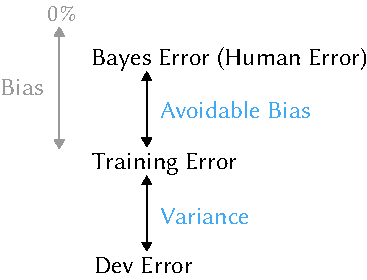
\includegraphics[width=6cm]{avoidable_bias.pdf}
    \caption{Avoidable Bias and Variance}
    \label{fig:avoidable_bias}
\end{figure}

\subsubsection{Understanding Human-level Performance}

在自然感知类任务上,例如图像分类、语音识别、文本分类等,
深度学习的方法很难达到人类的水平,人类的水平可以作为贝叶斯错误率的估计。
但在一些特定的任务上,例如广告推荐、搜索排序等,深度学习的方法已经超过了人类的水平,
在有大量数据的情况下,深度学习的方法可以达到很高的性能。

\subsubsection{Improving your Model Performance}

偏差大方差小说明模型拟合程度不足或训练不够充分;而偏差小方差大说明模型过拟合。

根据图~\ref{fig:avoidable_bias},确定可避免偏差和方差,并采取相应的措施:

\begin{enumerate}
    \item 如果可避免偏差较大,可以尝试以下选项:
        \begin{itemize}
            \item 训练更大的模型;
            \item 使用更好的优化算法(如 Momentum、RMSprop、Adam)进行更长时间的训练;
            \item 寻找更好的神经网络架构/超参数搜索。
        \end{itemize}
    \item 如果方差较大,可以尝试以下选项:
        \begin{itemize}
            \item 获取更多的训练数据;
            \item 正则化(如 L2、Dropout、数据增强);
            \item 寻找更好的神经网络架构/超参数搜索。
        \end{itemize}
\end{enumerate}

%%%%
\subsection{Error Analysis}

\subsubsection{Carrying Out Error Analysis}

有时候,模型可能在某些特定的方面表现不佳,例如在某些类别上分类错误率较高。
这时就需要引入\textbf{错误分析(Error Analysis)}。
错误分析是指对模型在开发集和测试集上的错误进行人工分析,
以了解模型在哪些方面表现不佳,从而改进模型。

例如,对于一个识别猫的模型,如果我们怀疑它在图片中含有狗,或者图片比较模糊的情况下分类错误率较高,
那么我们就可以对这些图片进行人工分析,随机取出 100 张标记错误的图片,看看其中有多少含有狗,或者图片是否比较模糊。
进行这样的计数可以帮助我们快速发现主要问题所在,从而有针对性地改进模型。

\subsubsection{Cleaning Up Incorrectly Labeled Data}

机器学习算法通常对于训练集中出现的\textbf{随机错误(Random Errors)}有较好的鲁棒性。
但是,如果训练集中存在\textbf{系统性错误(Systematic Errors)},例如某些特定类别的样本被错误地标记为其他类别,
那么这些错误可能会导致模型在训练过程中出现偏差,从而影响模型的性能。

在这种情况下,我们需要对训练集中的错误标记数据进行清理。同时,开发集和测试集也需要进行相应的清理,
以确保模型在开发和测试过程中不会受到这些错误标记的影响。如果训练集过大难以清理,至少也应当在开发集和测试集中进行清理。
就像前面提到的,开发集和测试集应当来自相同的分布,如果进行清理则两者都需要进行同样的清理。

\begin{hint}
    清理错误标记数据时,不仅要注意模型预测错误的样本,同时还要关注模型预测正确的样本。
    因为模型预测正确的样本也可能是错误标记导致的。
\end{hint}

\subsubsection{Build your First System Quickly, then Iterate}

在开发深度学习系统时,应该先快速构建一个基本的系统,然后进行迭代改进。
花费大量时间在构建一个不完善的系统上是不值得的。

%%%%
\subsection{Mismatched Training and Dev/Test Set}

\subsubsection{Training and Testing on Different Distributions}

很多时候,我们可能会收集到一些实际应用中的数据分布不一致的额外数据。
例如,想要开发一个通话语音识别的系统,我们的数据不太可能全部来自真实的通话数据。
我们可能会收集某视频网站的音频数据进行训练,然后在真实的通话数据上进行测试。
这时,训练集和开发/测试集就有了不一致的分布。

\ref{sec:train_dev_test_distributions} 节提到过,
开发/测试集必须对应到实际应用场景。这意味着如果你有 200000 条视频网站的音频数据,
却只有 10000 条通话数据,那么你不应将视频网站的音频数据添加到开发集和测试集中。
例如可以将 200000 条视频网站的音频数据和 5000 条通话数据作为训练集,
然后将 5000 条通话数据均分两部分作为开发集和测试集。

\subsubsection{Bias and Variance with Mismatched Data Distributions}

如果训练集与开发/测试集的分布不一致,
\ref{sec:comparing_to_human_level_performance} 节中提到的分析方法也要做进一步修正。
此时由于数据分布的差异,Training Error 和 Dev Error 之间的差距就不再是方差了。
此时可以引入一个 \textbf{Training-dev Set(训练-开发集)} 来辅助衡量方差。
训练-开发集与训练集遵循相同的分布,但不参与训练过程。

\begin{figure}[h!bt]
    \centering
    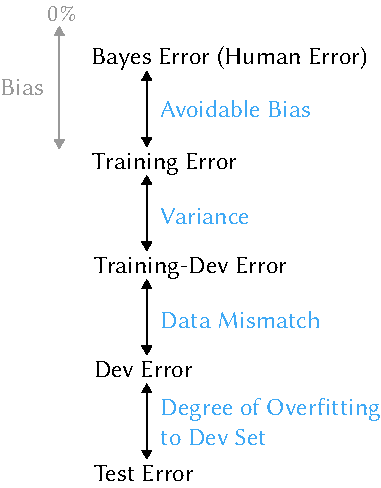
\includegraphics[width=6cm]{avoidable_bias_mismatched.pdf}
    \caption{Avoidable Bias and Variance with Mismatched Data Distributions}
    \label{fig:avoidable_bias_mismatched}
\end{figure}

如图~\ref{fig:avoidable_bias_mismatched}~所示,
添加训练-开发集后,训练集和训练-开发集间的差异可以用来衡量方差,
而训练-开发集和开发集间的差异可以反应数据失配的程度。
需要注意,图~\ref{fig:avoidable_bias_mismatched}~中从上到下的 Bayes Error、
Training Error、Training-dev Error、Dev Error 和 Test Error 并不一定是递增的,
在一些情形下,模型在开发和测试集上的表现可能比在训练集上还要好。

\subsubsection{Addressing Data Mismatch}

遗憾的是,解决数据分布失配问题并没有系统化的解决方案。
在实际应用中,可能需要靠一些洞察力和经验来观察和猜想问题的来源。
但最终的核心观念是缩小失配的程度,使训练集的数据更接近开发/测试集的数据分布。

例如在语音识别任务中,如果开发/测试集中的音频含有噪声,而训练集中是干净的音频,
此时可能需要对训练集进行数据增强,例如添加噪声,以提高模型在噪声环境下的表现。
再比如,一些合成的训练数据集可能多样性不足,只包含了少量的类别或特定的场景,
此时可能需要对训练集进行扩充,添加更多的类别或场景,以提高模型的泛化性。

%%%%
\subsection{Learning from Multiple Tasks}

\subsubsection{Transfer Learning}

\textbf{迁移学习(Transfer Learning)}是指在已经训练好的模型上进行微调,以适应新的任务。
模型在类似的任务上训练时,可能已经学习到了一些底层的低级特征,这些特征可以被用于新的任务上。
迁移学习可以利用已经训练好的模型的特征提取能力,减少训练时间,仅需要少量数据即可训练出一个性能良好的模型。

微调的方式一般是删除原模型的最后一层或几层,替换成能输出新任务所需特征的层(一般被称为任务头 head ),
然后在一个较低的学习率下重新训练模型。根据实际情况,可以冻结原模型的隐藏层,只训练任务头,
也可以同时训练原模型的隐藏层和任务头。

\subsubsection{Multi-Task Learning}

\textbf{多任务学习(Multi-Task Learning)}是指在同一个模型中同时学习多个相关任务。
多任务学习可以利用任务之间的相关性,提高模型的泛化能力。

例如,YOLO 模型可以同时检测物体和分类物体。在训练过程中,模型会同时学习物体检测和分类任务,
从而提高模型在两个任务上的表现。在实际应用中,多任务学习可以减少模型的复杂度,提高模型的泛化能力。

使用多任务学习需要满足几个条件:

\begin{enumerate}
    \item 任务之间存在相关性,有可以公用的低级特征;
    \item 任务之间使用的数据集可以共享;
    \item 有能力构建一个能够同时处理多个任务的大型模型。
\end{enumerate}

%%%%
\subsection{End-to-end Deep Learning}

\subsubsection{What is End-to-end Deep Learning?}
\index{End-to-end Learning}

在很多时候,人们倾向于把任务分解成多个子任务,从而降低实现的难度。
例如,在人脸识别中,人们可能会先进行人脸检测,框出人脸区域,然后再进行人脸的对比识别。

而\textbf{端到端深度学习(End-to-end Deep Learning)}是指在输入和输出之间没有中间步骤的深度学习模型。
这是一种“一步到位”的方法,可以避免中间步骤引入的误差,同时让模型自主发掘输入的隐藏特征。
例如,在语音识别中,端到端深度学习模型可以直接将音频信号映射到文字,而不需要进行中间的特征提取步骤。

\subsubsection{Whether to use End-to-end Deep Learning}

端到端学习的优缺点都很明显:

\begin{enumerate}
    \item 优点:
        \begin{itemize}
            \item 发挥数据本身的优势,让数据说话;
            \item 不需要人为设计特征,简化了工作流程。
        \end{itemize}
    \item 缺点
        \begin{itemize}
            \item 需要相对大量的数据,否则模型可能无法学习到有效的特征;
            \item 无法使用一些可以人为设计的先验知识和特征。
        \end{itemize}
\end{enumerate}

是否选择端到端学习的关键就是数据量的大小。
训练一个端到端深度学习模型需要大量的数据才能有效启发模型学习到有效的特征。
如果数据量不足,模型难以提取共性的低级特征,反而会陷入过拟合。
在数据不足的情况下,人为对任务进行辅助分解,依然是一个很好的选择。
